\documentclass[11pt, a4paper]{article}
\usepackage[utf8x]{inputenc}
\usepackage[sort]{natbib}

\usepackage[spanish]{babel}
\usepackage{enumitem}
\usepackage{graphicx}
\usepackage{float}

\usepackage{etoolbox}

\usepackage{amsmath}
\usepackage{array}
\usepackage{gensymb}

\usepackage{fancyhdr}
\usepackage{multirow}
\usepackage{multicol}
\usepackage[table]{xcolor}
\usepackage{color}
\usepackage{colortbl}
\definecolor{lightgray}{gray}{0.9}
\setlength{\columnsep}{0.5cm}

\usepackage{tikz}
\usetikzlibrary{shapes.geometric, arrows}
\tikzstyle{problema} = [rectangle, rounded corners,  minimum width=3cm, minimum height=1cm,text centered, draw=black,fill={rgb:black,1;white,30}]
\tikzstyle{causa} = [rectangle, minimum width=3cm, minimum height=1cm, text centered, text width=4cm, draw=black, fill={rgb:black,0;white,10}]
\tikzstyle{nodo} = [diamond, minimum width=1cm, minimum height=1cm, text centered, draw=black, fill={rgb:black,0;white,10}]
\tikzstyle{arrow} = [thick,->,>=stealth]


%------------------- Dimensiones -------------------
\usepackage{geometry}
 \geometry{a4paper,total={170mm,257mm},left=15mm,right=15mm,top=20mm,}
%----------------------------------------------------

%------------------- Encabezado y Pie de pág -------------------
\pagestyle{fancy}
\fancyhf{}
\lhead{Electrónica de Potencia}
\rhead{TP5 : Fuente conmutada ``Half Bridge"}
\rfoot{Página \thepage}
%----------------------------------------------------


%----------------------------- Documento -----------------------------------------------
\begin{document}
\begin{titlepage}
 \centering
	
\includegraphics[scale=0.80]{Imagenes/LOGO.jpg} \par
 	\vspace{1cm}
 	{\scshape\LARGE Universidad Tecnológica Nacional \par}
 	{\scshape\large Facultad Regional de Córdoba \par}
 	\vspace{1cm}
	{\bfseries \Large Trabajo Práctico De Laboratorio $N^{\circ} 5$\par}
	{\bfseries \Large Fuente conmutada ``Half Bridge" \par}
 	\vspace{1.5cm}

	\begin{tabular}{ll}
		Alassia, Francisco		&	60861	\\
		Amaya, Matías					&	68284	\\
		Lamas, Matías					&	65536 	\\
		Navarro, Facundo			&	63809 	\\
		Veron, Misael					&	62628
	\end{tabular}
	
	\vspace{1cm}
	Curso: 5r2 \\
	Grupo $N^{\circ} 11$
 	\vfill
	{\bfseries \Large Electrónica de Potencia \par}

	\vspace{1.5cm}
	Docentes: \par
	Ing. Oros, Ramón \par
	Ing. Avramovich, Javier \par

 	\vfill
	{\large \today\par}
\end{titlepage}
	
	
	\tableofcontents

%----------------your title below -----------------------------

\section{Introducción}
En el siguiente trabajo práctico se estudia el diseño y funcionamiento, a partir de su implementación, de una fuente de alimentación tipo off-line forward bidireccional en medio puente con las siguientes características:
\begin{itemize}
	\item Tensión de salida 24 V.
	\item Corriente de salida 2,5 A.
	\item Potencia de salida 60 W.
\end{itemize}

\section{Enunciado}
\begin{enumerate}
	\item Diseñar y construir una fuente de alimentación aislada de 60 W en lazo abierto. Especificaciones:
		\begin{enumerate}
			\item Convertidor medio puente bidireccional.
			\item Línea de alimentación: 200 a 240 $V_{RMS}$, 50 Hz.
			\item Frecuencia de conmutación: 80 KHz.
			\item Salida: 24 V, 2,5 A, límite de corriente 3,5 A.
			\item Salida: Ripple de 400 $mV_{PP}$, regulación en línea y carga $\pm$ 1\%.
			\item Circuito de protección contra sobre corriente. 
		\end{enumerate}
	\item Efectuar las siguientes mediciones:
		\begin{enumerate}
			\item Tensión y corriente de salida disponibles.
			\item Ripple a la máxima carga de salida.
		\end{enumerate}
\end{enumerate}


\section{Marco Teórico}
En primer lugar, se llama fuente de alimentación a todo circuito electrónico que convierte una tensión alterna de entrada en una tensión continua estable de salida, con el fin de proveer de energía de forma segura a otros circuitos.

Una fuente conmutada es un convertidor de energía DC/DC, cuya conmutación es producida por semiconductores de potencia, controlando la transferencia dinámica de potencia desde una fuente de entrada de DC hacia la carga, a través de conectar la fuente a la carga en transferencia directa o indirecta durante una duración de tiempo periódica y predeterminada.

\subsection{Clasificación}
Las fuentes conmutadas se pueden clasificar dependiendo de si tienen o no aislación galvánica entre la entrada de alimentación y el circuito de salida:
\begin{itemize} 
	\item \textbf{Convertidores NO asilados}
	
	Dependiendo del circuito de salida se clasifican en:
		\begin{itemize}
			\item Buck o reductoras.
			\item Boost o elevadoras.
			\item Buck/Boost o reductoras/elevadoras.
			\item $\acute{C}$uk.
			\item Zeta.
			\item SEPIC.
		\end{itemize}
	\item \textbf{Convertidores asilados}
	
	Según la excitación del núcleo magnético se clasifican en:
		\begin{itemize}
			\item Unidireccionales (permanecen en un solo cuadrante del ciclo magnético): dependiendo del circuito de salida pueden ser Forward o Flyback.
			\item Bidireccionales (trabajan en ambos cuadrantes del ciclo magnético): dependiendo de la configuración de los semiconductores de potencia pueden ser Push-Pull, Half-Bridge o Full-Bridge.
		\end{itemize}
\end{itemize}

\subsection{Ventajas y Desventajas}
Respecto a las fuentes lineales, las conmutadas presentan ciertas ventajas y desventajas que se mencionan a continuación.
\subsubsection{Ventajas}
\begin{itemize}
	\item Eficiencia entre el 68 y 90\%.
	\item Los dispositivos de potencia funcionan entre el corte y la saturación lo que aumenta su eficiencia.
	\item La tensión de entrada es conmutada en forma de alterna y ubicada en un elemento magnético, por lo que se puede variar la relación de transformación haciendo que la fuente funcione como reductor, elevador o inversor de tensión con múltiples salidas.
\end{itemize}
\subsubsection{Desventajas}
\begin{itemize}
	\item Diseño mas elaborado.
	\item Mayor ruido que en una fuente lineal. Entre entrada y salida hay interferencia electromagnética y de radiofrecuencias.
	\item Hay que agregar circuitos de protección como arranques suaves y filtros de línea lo que encarece a la fuente.
	\item Tiene una ``Respuesta transitoria en el tiempo". Lleva mayor tiempo de establecimiento al circuito el poder soportar variaciones en la tensión de entrada.
\end{itemize}

\subsection{Fuente de alimentación off-line forward bidireccional de medio puente}
A continuación se explica el funcionamiento y las características de la topología de fuente conmutada implementada en este trabajo práctico, la fuente conmutada asilada bidireccional Half-Bridge. (Figura \ref{halfbridge})

\subsubsection{Fuente off-line}
En la Fig. \ref{esquema} se observa la disposición de los elementos en una fuente conmutada off-line. El término off-line significa que el regulador (PWM) va en el primario del transformador de potencia y opera en forma independiente de la línea, aunque el regulador PWM puede estar conectado en el lado de la carga. Además, no utiliza transformador de alimentación adicional, ya que se rectifica la línea y se convierte a la tensión de salida $V_{out}$ sin utilizar transformador adicional.
\begin{figure}[h]
	\centering
	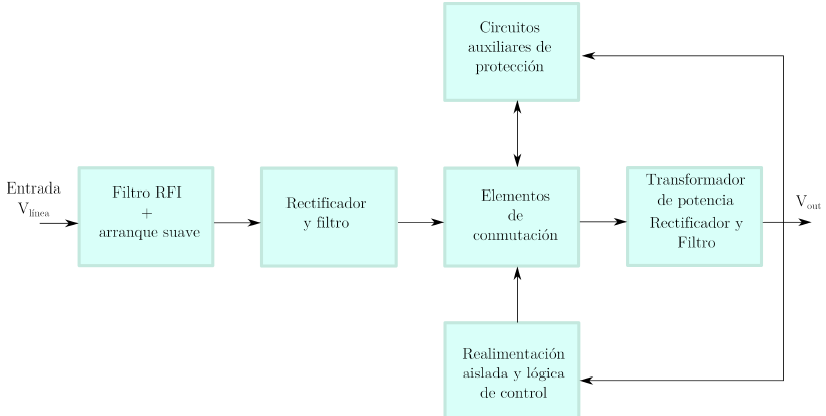
\includegraphics[width = 12 cm]{Imagenes/esquema}
	\caption{Diagrama en bloques de una fuente conmutada off-line.}
	\label{esquema}
\end{figure}

\subsubsection{Fuente Half-Bridge}
La topología de medio puente (Fig \ref{halfbridge}) es muy utilizada en convertidores off-line debido a que la tensión de bloqueo de los transistores es la de alimentación y no el doble de esta como en muchas otras topologías. La tensión máxima de los transistores será entonces:
\[V_{CEV} \; o \; V_{DSS} \geq V_{in_{MAX}} \]
Además, permite balancear los volts-segundo de cada transistor de conmutación automáticamente para prevenir la saturación utilizando un método sencillo de balanceo de intervalo de cada transistor sin emplear núcleos con entre hierro, y sin correctores de simetría.

\begin{figure}[h]
	\centering
	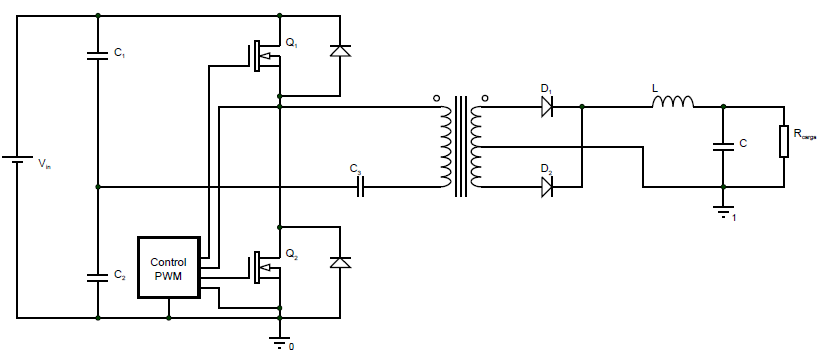
\includegraphics[width = 12 cm]{Imagenes/halfbridge}
	\caption{Esquemático de conexión de una fuente Half-Bridge.}
	\label{halfbridge}
\end{figure}

Esta topología es muy utilizada si la tensión de salida es de bajo valor. Se utiliza hasta los 500 W debido al valor grande que tendrían los capacitores de entrada en altas potencias.

A comparación de una fuente push pull, la half bridge puede entregar hasta el doble de corriente para una misma potencia de salida, debido a que cada transistor soporta menos tensión de bloqueo. Los transistores no pueden conducir simultáneamente, por lo que el ciclo de trabajo $D$ está limitado a los tiempos muertos necesarios $t_d$ entre conducción de cada transistor.
\[ D \leq 0,5 \]

\subsubsection{Transformador de potencia}
El objetivo del transformador de potencia es proveer aislación entre entrada y salida. El tamaño del transformador y su volumen, son inversamente proporcionales a la frecuencia de trabajo. Por lo que en fuentes conmutadas el tamaño de estos se ve considerablemente reducidos. Pueden tener múltiples devanados secundarios, lo que hace que la fuente tenga múltiples salidas.

\begin{figure}[h]
	\centering
	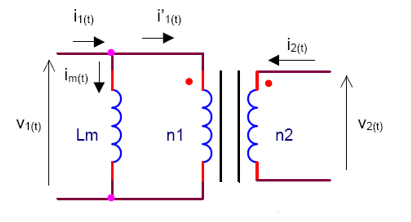
\includegraphics[width = 10 cm]{Imagenes/trafo}
	\caption{Transformador de Potencia.}
	\label{trafo}
\end{figure}

Como se observa en la Fig. \ref{trafo}, existe una inductancia en paralelo con el primario del transformador que es la inductancia de magnetización $L_m$. La corriente de magnetización $i_{Lm}$ que circula a través de esta es proporcional al campo magnético $H$ presente en el núcleo del transformador. Si esta corriente es muy grande, $H$ será tan grande que saturará al núcleo y $L_m$ se hace muy pequeña por lo que se pone en cortocircuito el transformador.

Para evitar este inconveniente la reactancia de magnetización $X_m$ debe ser muy grande en el rango de frecuencias de trabajo del transformador, para que la corriente de magnetización sea despreciable.
\[ i_{1}^{'} \gg i_m \; \rightarrow \; i_1 \tilde{=}  i_{1}^{'}  \]  

Por otro lado, $i_m$ es proporcional a la integral de la tensión aplicada en el primario, por lo que es importante que la componente de continua de dicha tensión sea nula, ya que de lo contrario en cada período de conmutación habría un incremento de la corriente que llevaría a la saturación del transformador.

\subsubsection{Funcionamiento}
Teniendo en cuenta el circuito de la Fig. \ref{propuesto}, las resistencias $R_1$ y $R_2$ conforman un divisor resistivo con el cual se obtiene la mitad de la tensión de entrada ${V_{in_{RMS}}}/{2} \; = 155 \; V$, que es el valor al cual los capacitores $C_1$ y $C_2$ se cargan. Estos son los encargados de almacenar la energía y proporcionar la corriente para el transformador cuando los MOSFET se habiliten.  

\begin{figure}[h]
	\centering
	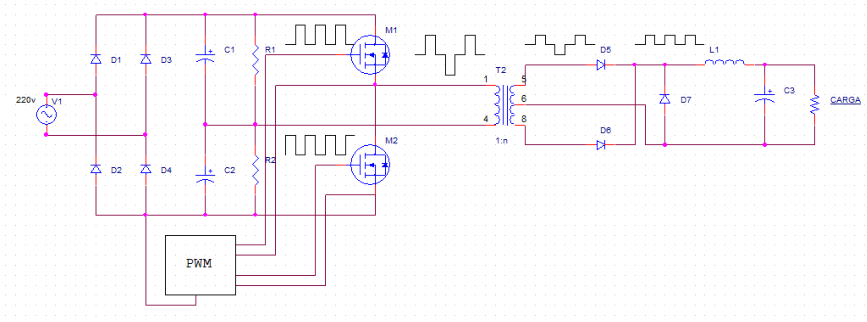
\includegraphics[width = \textwidth ]{Imagenes/funcionamiento}
	\caption{Circuito propuesto.}
	\label{propuesto}
\end{figure}

En este circuito se observa que el $PWM$ es el encargado de generar un tren de pulsos los cuales excitan el transistor $M_1$ y otro tren de pulsos desfasados $180^{\circ}$ para $M_2$. Los MOSFET trabajan en corte y saturacion con estados opuestos en el mismo instante. Los tiempos en el cual trabaja cada MOSFET se controlan regulando el duty en el PWM.

Luego de un tiempo fijado por el control (circuito PWM), el transistor $M_1$ conmuta a corte, mientras que $M_2$ pasa a conducción, invirtiendo la polaridad en los bornes del primario y circulando la corriente en sentido contrario.

En el primario del transformado es vista una tensión cuya forma de onda se muestra en la figura \ref{propuesto}, nótese que entre pulso positivo y negativo existe un tiempo el cero voltios o ``tiempo muerto", el cual es el tiempo en que los dos MOSFET se encuentran apagados simultáneamente. 

Una vez que la señal ingresa al transformador, éste con una adecuada relación de vueltas se encarga de reducir la tensión a la requerida, la forma de onda es de la misma naturaleza pero de menor amplitud.

Respecto al circuito de salida, como la fuente es tipo forward es derivada de las fuentes buck, por lo que es reductora. Observando el esquemático de una fuente buck (Fig. \ref{buck}) es posible analizar su funcionamiento.
\begin{figure}[h]
	\centering
	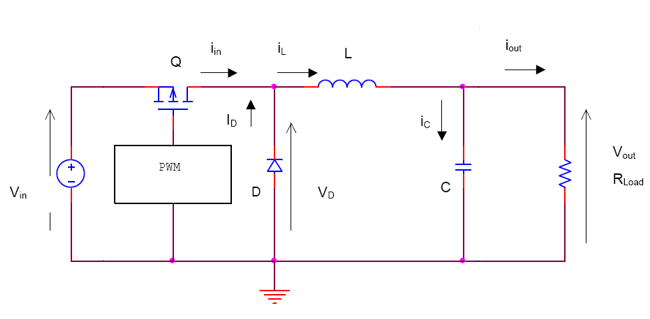
\includegraphics[width = 10 cm]{Imagenes/buck}
	\caption{Fuente conmutada buck.}
	\label{buck}
\end{figure}

Durante el $t_{on}$ (transistor saturado) se entrega energía a la carga a través de la inductancia que a su vez almacena energía. El diodo se encuentra polarizado inversamente por lo que no conduce y el capacitor esta para filtrar el ripple de la tensión de salida.

Durante el $t_{off}$ (transistor al corte) para evitar discontinuidades de corriente, el inductor invierte la polaridad en sus bornes haciendo que la corriente a través de el disminuya y polarizando directamente el diodo, el cual comienza a conducir y cierra el circuito para que haya entrega de energía a la carga.

Aplicando el funcionamiento antes mencionado a la fuente half-bridge, cuando $M_1$ está encendido la corriente del primer secundario circula por $D_5$ entregando energía a la carga. Cuando $M_1$ pasa a corte, la tensión en los bobinados se anula, pero la corriente deberá seguir circulando por los diodos del secundario forzada por la descarga de la corriente del filtro de salida. El comportamiento es similar cuando $M_2$ se satura, circulando la corriente por $D_6$.

Es importante que ambos bobinados secundarios tengan el mismo sentido de enrollamiento, para que la tensión en ellos tenga la misma polaridad de forma tal que conduzca cada diodo en un intervalo de conmutación distinto.

Se deduce del funcionamiento descrito que si se produce una conducción simultanea de $M_1$ y $M_2$, se produce un cortocircuito en la tensión de alimentación provocando la destrucción de los semiconductores.

\subsubsection{Modo de conducción discontinua DCM}
En caso de que la carga sea muy elevada puede suceder que la corriente que circula a través del inductor de salida sea menor a la mitad del ripple de esta misma, haciendo que el diodo se bloque antes de que comience un nuevo ciclo $t_{on}$, y por lo tanto anulando la corriente que circula a través del inductor de salida y por ende que se suministra a la carga.

Esto hace que las propiedades del convertidor cambien radicalmente respecto del modo de conducción continuo. La relación de conversión (función de transferencia) se hace dependiente de la carga y se incrementa la impedancia de salida.

\vfill
\section{Diseño de la fuente conmutada}
\subsection{Datos iniciales}
\begin{itemize}
	\item Tipo de Fuente: Half Bridge Forward Converter
	\item $V_{in} = 200$ a $240$ $V$ $\rightarrow$ $f_{in} = 50$ $Hz$
	\item $V_{out} = 24$ $V_{CC}$
	\item $I_{out} = 2,5$ $A$ $\rightarrow$ $I_{out_{max}} = 3,5$ $A$
	\item Ripple de tensión: $V_{ripple_{max}} = 400$ $mV_{PP}$
	\item Regulación en línea y carga: $\pm 1 \%$
	\item Eficiencia mínima: $\eta = 75 \%$
	\item Frecuencia de conmutación: $f_c = 80$ $KHz$
\end{itemize}
\subsection{Cálculos iniciales}
Los siguientes cálculos de potencia, corriente y tensión son los que regirán todo el diseño de la fuente conmutada:
\begin{itemize}
	\item Potencia de salida:
	\begin{equation}
	P_{out} = V_{out} \cdot I_{out}
	\label{Pout}
	\end{equation}
	\[ P_{out_{max}} = 24 \; V \cdot 3,5 \; A = 84 \;W \]
	\item Potencia de entrada:
	\begin{equation}
		P_{in_{max}} = \frac{P_{out_{max}}}{\eta}
	\label{Pin}
	\end{equation}
	\[ P_{in} = \frac{84 \; W}{0.75} \approx 107 \; W \]
	\item Tensión de entrada en continua $V_{in}$:
		\begin{itemize}
			\item Tensión de entrada máxima:
			\begin{equation}
				V_{in_{max}} = \sqrt{2} \cdot V_{RMS_{max}}
				\label{Vin_{max}}
			\end{equation}
			\[ V_{in_{max}} = \sqrt{2} \cdot 240 \; V = 339.41 \; V \]
			\item Tensión de entrada mínima:
			\begin{equation}
				V_{in_{min}} = \sqrt{2} \cdot V_{RMS_{min}}
				\label{Vin_{min}}
			\end{equation}
			\[ V_{in_{min}} = \sqrt{2} \cdot 200 \; V = 282.84 \; V \]
		\end{itemize}
	\item Corriente de entrada $I_{in}$:
	\begin{itemize}
		\item Corriente de entrada máxima:
		\begin{equation}
			I_{in_{max}} = \frac{P_{in_{max}}}{V_{in_{min}}}
			\label{I_{in{max}}}
		\end{equation}
		\[ I_{in_{max}} = \frac{107 \; W}{282.84 \; V} = 0.378 \; A \]
		\item Corriente de entrada mínima:
		\begin{equation}
			I_{in_{min}} = \frac{P_{in_max}}{V_{in_{max}}}
			\label{I_{in_{min}}}
		\end{equation}
		\[ I_{in_{min}} = \frac{107 \; W}{339.41 \; V} = 0.236 \; A \]
	\end{itemize}
\end{itemize}

\subsection{Circuito de Entrada de Línea - Filtro EMI/EMC}
La interferencia electromagnética es la perturbación que ocurre en cualquier circuito, componente o sistema electrónico causada por una fuente de radiación electromagnética externa o interna.
Al tener las fuentes conmutadas un circuito de conmutación, se genera interferencia eléctrica por conducción o radiación en la red de modo común y modo diferencial por las interrupciones en la corriente. Estas interferencias pueden causar fallas o mal funcionamiento en otros equipos conectados a la red. El filtro de línea tiene como objetivo absorber dichas interferencias generadas.

\begin{figure}[H]
	\centering
	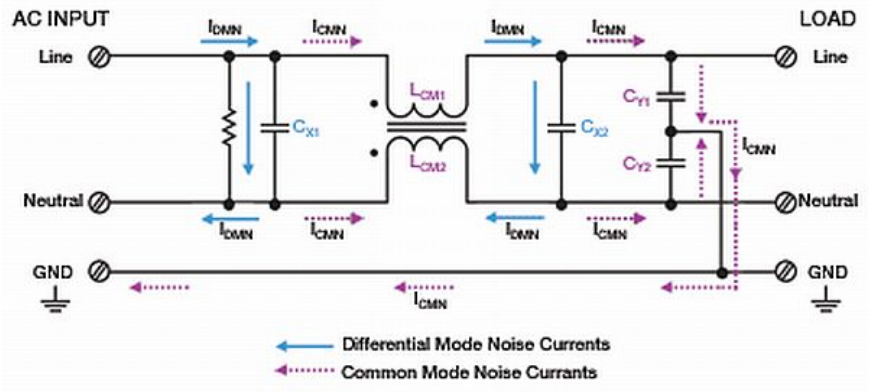
\includegraphics[scale = 0.4]{Imagenes/emi2}
	\caption{Circuito general de un filtro EMI.}
	\label{emi}
\end{figure}

	La mayoría de los circuitos AC/DC incorporan filtros EMI en el interior del gabinete para suprimir los ruidos e interferencias. Estos dispositivos se basan en sencillos circuitos inductivos que trabajan básicamente en ``modo diferencial", junto a capacitores que se colocan en paralelo con la linea de alimentación de red. Los circuitos más elaborados, de mayor calidad y costo, incorporan ademas capacitores referidos a masa que tienen la propiedad de filtrar los ruidos y poseen una operación denominada en ``modo común". 

Mas allá de las características funcionales del filtro EMI su aplicación es consecuencia directa de normas de diseño nacional e internacional para dispositivos que utilicen conmutación o sean susceptibles de generar interferencia hacia otros dispositivos.

En la Fig. \ref{emi} se observa el esquemático de conexión del filtro EMI implementado.

\begin{figure}[h]
	\centering
	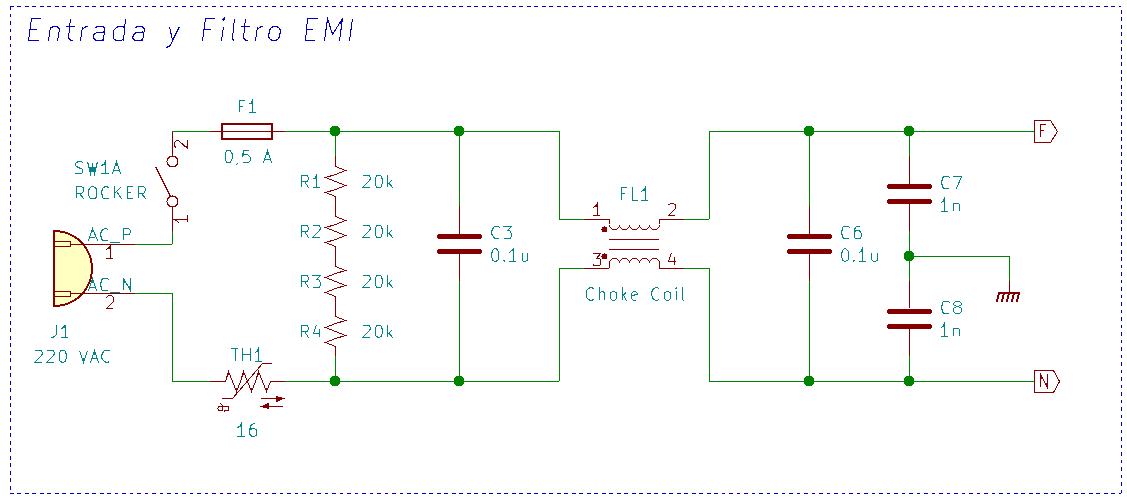
\includegraphics[width = \textwidth]{Imagenes/emi}
	\caption{Filtro EMI.}
	\label{emi}
\end{figure}

En la práctica el filtro EMI fue implementado a partir de otro filtro obtenido de una fuente de alimentación de un impresora.

\subsection{Circuito de Rectificación}
Las fuentes conmutadas son convertidores DC/DC, por lo que la tensión de red debe ser previamente rectificada y filtrada con una amplitud de rizado aceptable.

La etapa de rectificación se encarga de convertir la tensión alterna de la línea en tensión continua. Para ello se utiliza un rectificador de onda completa y un conjunto de capacitores que actúan de filtro disminuyendo el ripple. Al utilizar dos capacitores idénticos en serie, el circuito permite obtener un punto donde la tensión continua es la mitad de la de entrada ($V_{in}/2$), que es utilizada después para el funcionamiento del medio puente en la etapa de potencia. En la Fig. \ref{rectificador} se muestra el circuito de rectificación.

\begin{figure}[h]
	\centering
	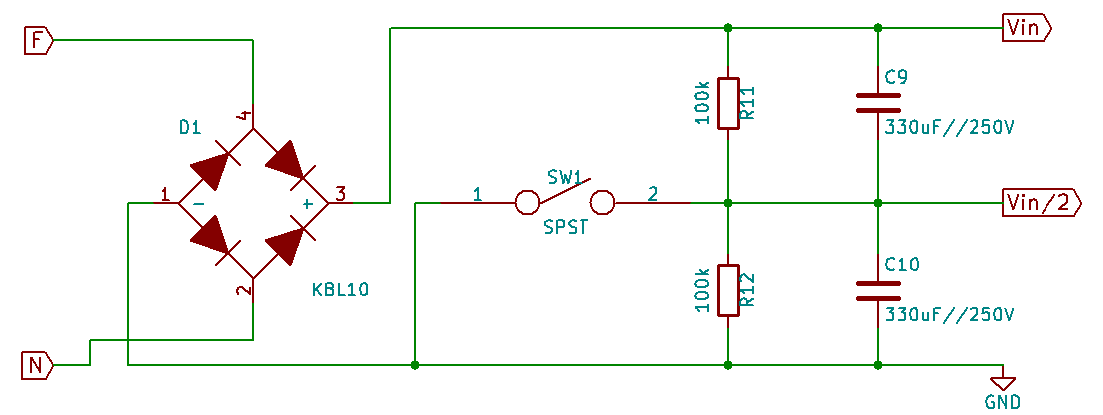
\includegraphics[width = \textwidth]{Imagenes/rectificador}
	\caption{Etapa rectificadora.}
	\label{rectificador}
\end{figure}

Las resistencias en paralelo a los capacitores deben ser del orden de los $K\Omega$, para que los capacitores se descarguen y para que las resistencias no disipen mucha potencia.

\subsubsection{Puente Rectificador}
Para elegir el puente rectificador a utilizar (o los diodos para armarlo), pueden hacerse estimaciones en base a cálculos de la corriente de entrada y las potencias necesarias para el proceso de conversión. El transformador debe cumplir con la ``Ley de conservación de energía" y por tanto si su tensión de entrada es grande, de modo de mantener la relación de potencia, su corriente de entrada debe ser pequeña. Del análisis anterior se saco la corriente máxima de entrada. 


\[ I_{in_{max}} = \frac{107 \; W}{282.84 \; V} = 0.378 \; A \]


De forma de poder garantizar la durabilidad del componente y evitar el estrés térmico y de tensión inversa aplicada se selecciona una corriente de funcionamiento nominal máximo para el puente como:

\[ I_{rectificador} \geq 3 \cdot I_{in_{max}} \approx 1 \;A \]

El puente rectificador puede ser implementado por cuatro diodos 1N4007 o por el puente integrado KBL06/08/10. En este práctico se implementó el D3SB60 que cumple con los requisitos anteriores, por estar reciclado de la misma fuente de la cual se saco el filtro EMI.

\subsubsection{Capacitores y Resistencias de Filtro}
El valor de los capacitores de filtro viene dado por la expresión \ref{capf}, donde $I$ es la corriente de entrada máxima, $t$ es el tiempo en que se suministra dicha corriente y $\Delta V$ es el ripple de tensión máximo. 
\begin{equation}
C = \frac{I \cdot t}{\Delta V}
\label{capf}
\end{equation}
\[ \Delta V = 10 \; V \]
\[ t = \frac{1}{2 \cdot f_{in}} = \frac{1}{2 \cdot 50 \; Hz} = 0.01 \; seg\]
\[ C_9 = C_{10} = \frac{0.283 \; A \cdot 0.01 \; seg}{10 \; V} = 283 \; \mu F \]

Al ser los dos capacitores de mismo valor, se encuentran formando un divisor de tensión, por lo que la tensión que soporta cada uno de ellos es:
\begin{equation}
V_{Cmax} = \frac{V_{inmax}}{2}
\label{VCMAX}
\end{equation}
\[ V_{Cmax} = \frac{339.41 \; V}{2} = 169.705 \; V \]

Llevando a valores comerciales lo calculado anteriormente, se define el uso de los siguientes capacitores:
\[ C_9 = C_{10} = 330 \; \mu F / \geq 200 \;V \]

Definiendo $R_{11} = R_{12} = 100$ $K\Omega$, la potencia que disiparan dichas resistencias será:
\begin{equation}
P_{R11-12} = \frac{V_{Cmax}^2}{R_{11}}
\label{PR1112}
\end{equation}
\[ P_{R11-12} = \frac{(169.705 \; V)^2}{100 \; K\Omega } = 0.288 \; W \]

Llevando a valores comerciales lo calculado anteriormente, se define el uso de las siguientes resistencias:
\[ R_{11} = R_{12} = 100 \; K\Omega / 0.5 \;W \]

\subsection{Circuito generador del PWM}
El PWM se implementa con el circuito integrado SG3525 (Fig. \ref{pwm}), el cuál opera a una frecuencia fija que es programada a través de la relación entre la resistencia $R_T$ ($R_{V2} + R_{18}$), $R_D$ ($R_{20}$) y el capacitor $C_T$ ($C_{15}$). Con este integrado se genera un tren de pulsos cuadrados, utilizando una tensión continua ($12$ $V$) y con la posibilidad de regular el ciclo de trabajo por medio de $R_{V1}$.

\begin{figure}[h]
	\centering
	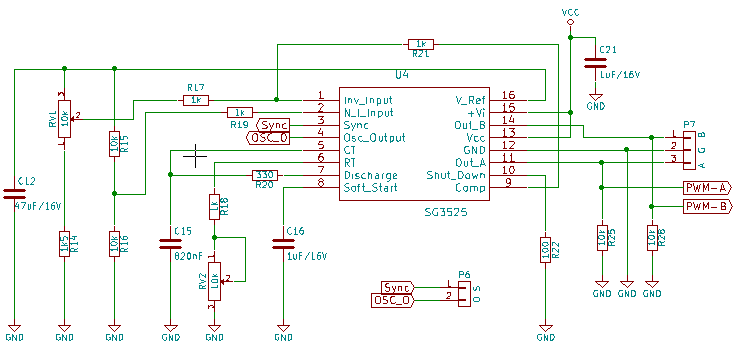
\includegraphics[width = 12 cm]{Imagenes/PWM}
	\caption{Circuito generador del PWM.}
	\label{pwm}
\end{figure}

La frecuencia de oscilación del PWM está definida por la ecuación \ref{fpwm}. Definiendo $C_T = 820$ $pF$ y $R_D = 330$ $\Omega$ podemos determinar el valor de $R_T$ (ecuación \ref{RT}) para la frecuencia de conmutación deseada $f_c = 80$ $KHz$.

\begin{equation}
f_c = \frac{1}{2 \cdot C_T \cdot (0.7 \cdot R_T + 0.3 \cdot R_D)}
\label{fpwm}
\end{equation}
\begin{equation}
R_T = \frac{1}{0.7} \cdot (\frac{1}{2 \cdot f_c \cdot C_T \cdot} - 0.3 \cdot R_D)
\label{RT}
\end{equation}
\[ R_T = \frac{1}{0.7)} \cdot (\frac{1}{2 \cdot 80 \; KHz \cdot 820 \; pF \cdot} - 0.3 \cdot 330 \; \Omega) = 10.747 \; K\Omega \]

La resistencia $R_T$ se forma con un potenciómetro en serie con una resistencia ($R_{V2} + R_{18}$) para poder ajustar la frecuencia de conmutación al valor deseado.

La resistencia $R_D$ es la encargada de garantizar la existencia de un tiempo muerto entre cada flanco de disparo de la señal de salida del PWM. Este tiempo muerto es necesario para la conmutación de los transistores de potencia de la fuente conmutada, para evitar que haya conducción simultanea de estos y se produzca un cortocircuito que lleve a la destrucción de los dispositivos de potencia. El tiempo muerto se elije como 10 veces el tiempo de apagado de los transistores utilizados.

\subsection{Selección del dispositivo de conmutación}
Debido a la frecuencia de conmutación se utilizan transistores MOSFET de potencia que cumplan con las siguientes características:
\subsubsection{Encendido o Saturación}
En este momento la corriente a través del dispositivo es máxima y depende de la corriente máxima de entrada y del ciclo de trabajo de los transistores.
\begin{equation}
I_{Dmax} = \frac{I_{inmax}}{D}
\label{IDmax}
\end{equation}
\[ I_{Dmax} = \frac{0.283 \; A}{0.45} = 0.623 \; A \]

\subsubsection{Apagado o Corte}
En este momento el transistor debe soportar la tensión de entrada máxima.
\begin{equation}
V_{DSSmax} = V_{inmax}
\label{VDmax}
\end{equation}
\[ V_{DSSmax} = 339.41 \; V \]

Con las características antes definidas se puede seleccionar como elemento conmutado a los transistores MOSFET IRF830/840. ($V_{DSSmax} = 500 \; V$, $I_{Dmax} = 4.5/8 \; A$)

\subsection{Driver de los MOSFET}
La señal del generador de PWM, no puede ser aplicada directamente a los transistores de conmutación, ya que se necesitaría referenciar la señal a niveles altos de tensión para lograr una correcta $V_{GS}$ que permita
encender los MOSFETs. Por esta razón se coloca un circuito driver intermedio, que entre otras funciones, adapta los niveles de tensión.

\subsubsection{IR2110}
Como driver de los transistores de tensión se puede utilizar un transformador de aislación como se hizo en el trabajo práctico N°3 de la materia, o un circuito integrado, el IR2110.

El IR2110 es un driver de alta velocidad y potencia integrado, que obtiene los niveles de tensión necesarios para disparar un transistor de conmutación mediante un capacitor y un diodo en configuración $Bootstrap$. 

En la Fig. \ref{driver} se observa el circuito de driver de los MOSFETS que forman el medio puente. El circuito integrado entrega la tensión suficiente para saturar el transistor correspondiente cuando en cualquiera de sus dos entradas ($HIN$ o $LIN$) exista un nivel alto. Este circuito se obtuvo de la nota de aplicación del IR2110.

\begin{figure}[h]
	\centering
	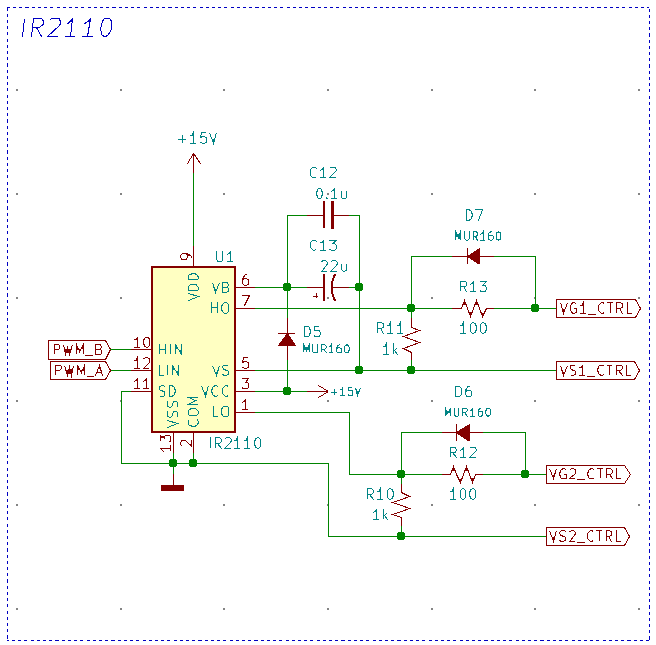
\includegraphics[width = 12 cm]{Imagenes/driver}
	\caption{Circuito driver de los MOSFETs implementado con IR2110.}
	\label{driver}
\end{figure}

La configuración $Bootstrap$ formada por el diodo $D_5$ y el capacitor $C_{17}$ tiene como objetivo elevar el punto de operación del transistor superior, es decir, entrega una tensión flotante entre la salida superior $HO$ y el punto medio entre los transistores $VS$. Cuando se satura el transistor inferior, la tensión en $VS$ es puesta a $0$ $V$ y el capacitor se carga a $V_{CC}$ a través del diodo. Cuando el mismo transistor está en corte, el capacitor entrega la tensión flotante y el diodo impide que la corriente se vaya a través de $V_{CC}$, posibilitando así disparar el transistor superior del medio puente.

De acuerdo con la nota de aplicación del IR2110, el capacitor de $Bootstrap$ se calcula con la ecuación \ref{CBS}, donde $Q_g$ es la carga necesaria en la compuerta del MOSFET, $f$ la frecuencia de operación, $I_{Cbs(leak)}$  es la corriente de pérdida del capacitor de $Bootstrap$, $I_{qbs(max)}$ es la máxima corriente de reposo, $V_{CC}$ la tensión de alimentación del integrado, $V_f$ la caída de tensión en el diodo de $Bootstrap$ en directa, $V_{LS}$ la caída de tensión en el MOSFET inferior, $V_min$ la tensión $V_BS$ mínima y $Q_ls$ el nivel de carga requerido por ciclo.

\begin{equation}
C_{BS} \geq \frac{ 2 \cdot [2\cdot Q_g + \frac{I_{qbs(max)}}{f} + Q_ls + \frac{I_{Cbs(leak)}}{f}]}{V_{CC} - V_f - V_{LS} - V_{min}}
\label{CBS} 
\end{equation}

\[ C_BS \geq \frac{ 2 \cdot [2\cdot 32nC + \frac{230 \mu A}{80 KHz} + 5 nC + \frac{despreciable}{80 KHz}]}{15 V - 1.25 V - 10 V - 0 V} \geq 38.33 \; nF \]

Los valores anteriores se toman de la hoja de datos del transistor utilizado y de la nota de aplicación del IR2110. Así mismo,la nota indica que el diodo a utilizar para $Bootstrap$ es el $MUR160$ ($D_5$) y que el capacitor debe ser al menos unas 15 veces mas grande al valor calculado por lo que se usa un capacitor de $4.7$ $\mu F\; /\; 16$ $V$ ($C_{17}$).

Los diodos $D_6$ y $D_7$ son 1N4148 (nota de aplicación) y tienen como objetivo acelerar el proceso de apagado del transistor ya que ayudan "quitando" cargas del gate.

El criterio de selección del diodo de $Bootstrap$, de acuerdo a la nota de aplicación, es que el tiempo de recuperación inversa ($t_r$) de dicho diodo debe ser mas rápido que el período de conmutación de los transistores ($1/f_c$).

\subsubsection{Velocidad de Conmutación}
La velocidad de conmutación no solo depende de los transistores empleados sino también del driver que los maneja. Para los MOSFET de potencia están bien definidas la características que debe cumplir el driver para obtener las velocidades de conmutación deseadas.

Empleando la curva de $V_{GS} = f(Q_G)$ (Fig. \ref{vgsfqg}), que muestra la carga que va acumulando el gate durante todo el proceso de conmutación para una corriente $I_G$ constante, se puede obtener la corriente $I_G$ requerida para satisfacer los requerimientos de velocidad.

\begin{figure}[h]
	\centering
	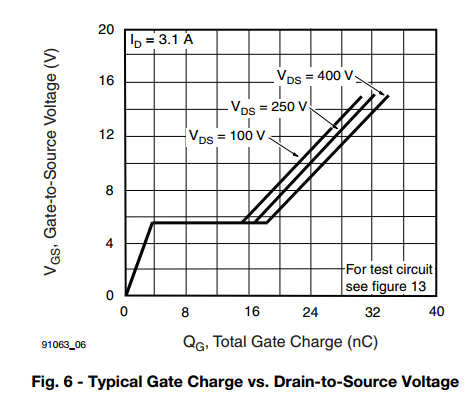
\includegraphics[width = 10 cm]{Imagenes/vgsfqg}
	\caption{$V_{GS}$ vs $Q_G$.}
	\label{vgsfqg}
\end{figure}

Se observa que para $V_{GS} = 15$ $V$ y $V_{DS} = 250$ $V$ $Q_G = 32$ $nC$. Esto nos permite calcular la corriente de gate $I_G$ (ecuación \ref{IG}) que debe suministrar el driver, analizando previamente el tiempo de conmutación de los transistores a partir de su hoja de datos y de la ecuación \ref{tc}.

\begin{equation}
t_c = t_{on} t_{off} = t_{don} + t_{r} + t_{doff} + t_f
\label{tc} 
\end{equation}

\[ t_c = 8,2 \; ns\; + 16 \; ns\; + 42 \; ns\; + 16 \; ns\; = 82.2 \; ns \tilde{=} 100 \; ns \]

\begin{equation}
I_G = \frac{Q_G}{t_c} 
\label{IG} 
\end{equation}

\[ I_G = \frac{32 \; nC}{100 \; ns} = 0.32 \; A \]

El driver IR2110 entrega picos de corriente de hasta $2$ $A$ durante intervalos de $10$ $\mu s$, es decir que cumple con los requisitos para la conmutación de los MOSFETs.

Se procede a calcular la potencia que debe entregar el driver para conmutar los transistores y la resistencia de gate necesaria para lograr la $I_G$ deseada, a partir de la Fig. \ref{vgsfqg}.

\[ P_{driver} = Q_G \cdot V_{GS} \cdot f_c = 32 \; nC \cdot 15 \; V \cdot 80 \; KHz = 38.4 \; mW \]

\[ R_G = \frac{V_{GS(sat)} - V_{GS(plana)}}{I_G} = \frac{15 \; V - 5.5 \; V}{0.32 \; A} = 30 \; \Omega  \]

\subsection{Transformador de Potencia}
A continuación se realizan los cálculos y aclaraciones necesarias para garantizar que el núcleo empleado en el armado del transformador de potencia funcionará correctamente para lo que es diseñado.
\subsubsection{Material y Cazoleta}
El núcleo empleado es el $E20/10/6$ material $N27$ de EPCOS.
\begin{itemize}
	\item $A_L = 1300$ $nHy$
	\item $\mu e = 1490$
	\item $\mathit{l}_e = 46.3$ $mm$
	\item $A_e = 32.1$ $mm^2$
	\item $A_min = 31.9$ $mm^2$
	\item $V_e = 1490$ $mm^3$
	\item Dimensiones: 23 x 22.2 x 16.8 mm  
\end{itemize}
\subsubsection{Excursión de la densidad de flujo}
El transformador se deberá diseñar para operar en el mayor valor de $\Delta B$ posible, resultando en una cantidad de vueltas menor en el devanado, incrementando el rango de potencia y obteniéndose menores pérdidas de inductancia debidas al devanado. El valor máximo de $\Delta B$ está limitado por el valor de saturación.

\begin{figure}[h]
	\centering
	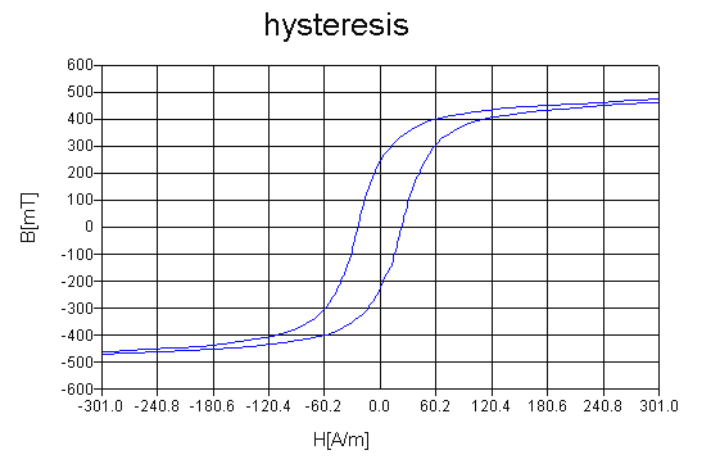
\includegraphics[width = 10 cm]{Imagenes/n27}
	\caption{Curva de histéresis del material N27.}
	\label{n27}
\end{figure}

La Fig. \ref{n27} muestra la curva de histéresis del material de la cazoleta empleada. Para el diseño se determina un $\Delta B = 300$ $mT$.
\subsubsection{Comprobación del tamaño de la cazoleta}
Este es un procedimiento iterativo que permite seleccionar un núcleo específico que sea capaz de soportar los voltios por segundos sin saturarse y con pérdidas en el núcleo y en el devanado aceptables. 
Un método útil es aplicar la ecuación del “área de producto $AP$” (ecuación \ref{AP}) que es el producto del área de la ventana del núcleo $A_W$ multiplicada por el área efectiva del núcleo $A_e$ . 

Para calcular el área de ventana necesitamos las dimensiones del núcleo a utilizar (Fig. \ref{cazoleta}), teniendo en cuenta que se utilizan dos de ellos enfrentados.

\begin{figure}[h]
	\centering
	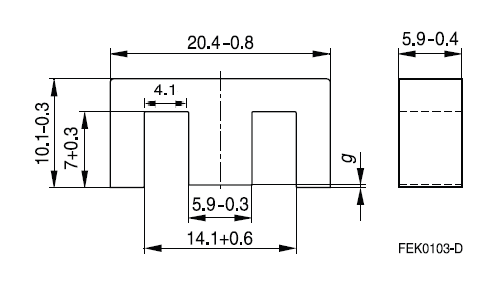
\includegraphics[width = 10 cm]{Imagenes/cazoleta}
	\caption{Dimensiones del núcleo utilizado.}
	\label{cazoleta}
\end{figure}

\begin{equation}
AP = A_w \cdot A_e
\label{AP}
\end{equation}
\[ AP = 2\cdot 4.1 \; mm \; \cdot 7 \; mm \cdot 32.1 \; mm^2 = 182.54 \; mm^4 \; = 0.18254 \; cm^4 \]

El valor de $AP$ del núcleo seleccionado deberá ser mayor o igual a $AP^{'}$ (ecuación \ref{AP'}), que es otra forma de calcular el área de producto cuando el valor de $\Delta B$ está limitado por el valor de saturación, de lo contrario el núcleo no será el adecuado para esta aplicación.

\begin{equation}
AP^{'} = [\frac{P_{out} \cdot 10^4}{\eta \cdot K_t \cdot K_u \cdot K_p \cdot 420 \cdot \Delta B \cdot 2 \cdot f_c}]^{1.31}
\end{equation}
\[ AP^{'} = [\frac{60 \; W \; \cdot 10^4}{0.75 \cdot 0.165 \cdot 420 \cdot 300 \; mT \; \cdot 2 \cdot 80 \; KHz}]^{1.31} = 0.1546 \; cm^4 \]
Donde:
\begin{itemize}
	\item $P_{out}$: potencia de salida.
	\item $K_t = \frac{I_{entrada}}{I_{primario}}$: depende de la topología.
	\item $K_u = \frac{A^{'}_w}{A_w}$: factor de utilización de la ventana.
	\item $K_p = \frac{A_p}{A^{'}_w}$: factor de área del primario. 
\end{itemize}

$K_u$ es la fracción del área de la ventana del núcleo que está llenada ahora con el bobinado. Se reduce por la aislación, por la distancia en el final del recorrido de la bobina en aplicaciones de alta tensión, y por el factor de llenado (forma del área del cableado y capas). Varía típicamente entre $0.4$ y $0.3$ en fuentes off-line de alta aislación.

$K_p$ es el área relativa del primario respecto al área total de todos los devanados, proporcionados de manera tal que todos los devanados operen a la misma densidad de corriente RMS y la misma densidad de potencia.

La siguiente tabla muestra valores típicos de las constantes K para distintas topologías de fuentes conmutadas, donde SE/SE: single ended primary \& secundary, SE/CT: Single endend primary \& center tap secundaries y CT/CT: center tap primary \& secundaries:
\begin{center}
	\begin{tabular}[h]{|c|c|c|c|c|c|}
		\hline
		 & & $K$ & $K_t$ & $K_u$ & $K_p$ \\
		 \hline
		 Forward & SE/SE & 0.141 & 0.71 & 0.40 & 0.50 \\
		 Full/Half Bridge & SE/CT & 0.165 & 1.0 & 0.40 & 0.41 \\ 
		 Full wave center tap & CT/CT & 0.141 & 1.41 & 0.40 & 0.25\\
		 \hline
	\end{tabular}
\end{center}

\begin{equation}
\Delta P > \Delta P_{'}
\label{AP'}
\end{equation}

\[ 0.18254 cm^4 > 0.1546 \; cm^4 \]

\subsubsection{Número de vueltas del primario y del secundario}
Para calcular el número de vueltas del primario se utiliza la ley de Faraday modificada (ecuación \ref{Np}), donde $\hat{V}_p$ es la tensión pico de entrada del primario ($Vin/2$), $A_{min}$ es el área efectiva mínima de la cazoleta, $\Delta B_{max}$ es la máxima variación de flujo permitida y $f_c$ la frecuencia de conmutación.
\begin{equation}
	N_p \geq \frac{0.225 \cdot \hat{V}_p \cdot 10^9}{f_c \cdot \Delta B_{max}} \cdot A_{min} 
	\label{Np}
\end{equation}
\[ N_p \geq \frac{0.225 \cdot 160 \; V \; \cdot 10^9}{80 \; KHz \; \cdot 300 \; mT \; \cdot 31.9 \; mm^2} = 46.72 \; vueltas = 47 \; vueltas \]

Para calcular el número de vueltas del secundario se tiene en cuenta la relación de transformación del transformador. La ecuación utilizada es la ecuación \ref{Ns}, donde $V_o$ es dos veces la tensión de salida de la fuente, $V_d$ dos veces la caída de tensión del rectificador de salida, $V_i$ la tensión de entrada del primario y $N_p$ el número de vueltas del primario.

\begin{equation}
	N_s \geq \frac{(V_o + V_d) \cdot N_p}{V_i}
	\label{Ns}
\end{equation}
\[ N_s \geq \frac{(48 \; V \; + 1.4 \; V) \cdot 47 \; vueltas}{160 \; V} = 14.51125 \; vueltas = 15 \; vueltas \; por \; secundario \]

\subsubsection{Diámetro de los conductores}
Suponiendo una densidad de corriente $J = 4.2$ $A/mm^2$, el diámetro de los conductores se calcula como en \ref{diamprimario} y \ref{diamsecundario} :
\begin{itemize}
	\item Primario:
		\begin{equation}
		\phi_P = \sqrt{\frac{4 \cdot I_{Dmax}}{\pi \cdot J}}
		\label{diamprimario}
		\end{equation}
		\[ \phi_P = \sqrt{\frac{4 \cdot 0.623 \; A}{\pi \cdot 4.2 \; A/mm^2}} = 0.434 \; mm = 0.45 \; mm \]
	\item Secundario: este está dividido en dos.
		\[ I_{RMS} = I_{out} \cdot \sqrt{\frac{D_{max}}{2}} = 2.5 \; A \; \cdot \sqrt{\frac{0.9}{2}} = 1.677 \; A \]
		\begin{equation}
		\phi_P = \sqrt{\frac{4 \cdot I_{RMS}}{\pi \cdot J}}
		\label{diamsecundario}
		\end{equation}
		\[ \phi_P = \sqrt{\frac{4 \cdot 1.677 \; A}{\pi \cdot 4.2 \; A/mm^2}} = 0.713 \; mm = 0.8 \; mm \]
\end{itemize}

\subsubsection{Capacitor de acople $C_{14}$}
El capacitor de acople se coloca porque siempre existe una diferencia de tensión, por las tolerancias de los componentes, que tiene como consecuencia la existencia, entre los terminales del primario del transformador, de un valor de continua que lleva al núcleo a la saturación. 

Este capacitor de acoplamiento es normalmente del tipo sin polaridad capaz de manejar la corriente del primario. Deberá, además, tener un valor bajo de $ESR$ para evitar el calentamiento.

Debido a que el capacitor se carga y descarga todos los semiciclos de la frecuencia de conmutación, la componente en continua se adicionará a $Vin / 2$.

La tensión de carga del capacitor es:
\begin{equation}
\Delta V_C = \frac{I_{Dmax} \cdot t}{C}
\label{VC}
\end{equation}
\[ t = t_on = \frac{1}{f_c} \cdot D = \frac{0.45}{80 \; KHz} = 5.625 \; \mu s \]
\[ \Delta V_C = 10 \; al \; 20 \% \; Vin / 2 \rightarrow 17 \; V < \Delta V_C < 34 \; V \]

\begin{equation}
C =  \frac{I_{Dmax} \cdot t}{\Delta V_C}
\label{C}
\end{equation}
\[ C =  \frac{0.623 \; A \; \cdot 5.625 \; \mu s}{\Delta V_C} \rightarrow 103.07 \; nF \; < C < 206.14 \; nF \]

\[ C_{14} = 120 \; nF \; / \; 400 \; V \]

\subsection{Circuito de salida}
En la etapa de salida se utiliza nuevamente un rectificador junto a un
filtro, para convertir la corriente alterna pulsante (generada en la etapa de conmutación) en corriente continua de salida. Para ello se emplea EL circuito presentado en la Fig. \ref{salida}.

\begin{figure}[h]
	\centering
	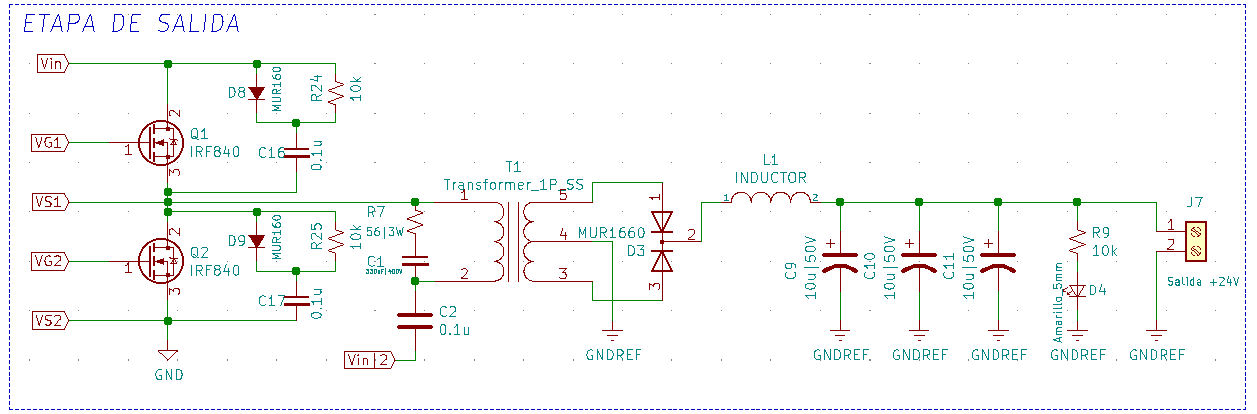
\includegraphics[width = 12 cm]{Imagenes/trafo_salida}
	\caption{Etapa de salida.}
	\label{salida}
\end{figure}

\subsubsection{Rectificadores}
Para elegir los diodos rectificadores de salida, se debe tener en cuenta la corriente máxima en directa y el tiempo de recuperación inversa. Esto último es importante, ya que dada la alta frecuencia de la corriente, no es posible utilizar diodos rectificadores comunes. De hacerlo estos tardarían demasiado tiempo en dejar de conducir. Por ello se utilizan diodos rápidos de potencia.

La corriente media por los diodos está definida como la mitad de la corriente máxima de salida:
\begin{equation}
I_{F(AV)} \geq \frac{I_{omax}}{2} \geq \frac{3.5 \; A}{2} \geq 1.75 \; A
\end{equation}

El tiempo de recuperación inversa debe ser menor a:

\begin{equation}
t_r \leq \frac{1}{f_c} \leq \frac{1}{80 \; KHz} \leq 1.25 \; \mu s
\end{equation}

La tensión pico inversa debe ser mayor a:
\begin{equation}
V_{RRM} \geq \frac{(V_o + V_F) \cdot V_{inmax} }{D_{max} \cdot V_{inmin}} \geq 33 \; V
\label{VRDO}
\end{equation}

Se utiliza el MUR1640.

\subsubsection{Inductor}
El inductor operará con CC superpuesta que no se anulará, y además, trabajará en un sólo cuadrante del ciclo B-H. Típicamente se diseña con una capacidad del 50\% mas que la que requiere la carga, durante el ciclo de operación.

Para determinar la inductancia necesaria se deben tener en cuenta la energía almacenada en el inductor por ciclo \ref{AE}, la energía remanente en el núcleo \ref{ER} y la frecuencia aplicada al inductor \ref{toff}.

\begin{equation}
\Delta E = \frac{1}{2} \cdot L \cdot (i_{pk} - i_{min})^2 
\label{AE}
\end{equation}

\begin{equation}
E_r = \frac{1}{2} \cdot L \cdot (i_{min})^2 
\label{ER}
\end{equation}

\begin{equation}
T_{offmax} = \frac{1 - \frac{V_{out}}{V_{in}}}{2\cdot f_c} = \frac{1 - \frac{24 \; V}{48 \; V}}{2\cdot 80 \; KHz} = 3.125 \; \mu s
\label{toff}
\end{equation}

A partir de la ecuación \ref{L} , que establece la relación de tensión y corriente en un inductor se calcula el valor de la inductancia.

\begin{equation}
L = \frac{V_o \cdot T_{offmax}}{0.25 \cdot I_o} = \frac{24 \; V \cdot 3.125 \; \mu s}{0.25 \cdot 2.5 \; A} = 120 \; \mu Hy
\label{L}
\end{equation}

La energía que deberá almacenar el inductor será:
\[ E = \frac{1}{2} \cdot L \cdot I_{o}^{2} = 375 \mu J \]

Con este dato se procede a elegir el núcleo del toroide. El núcleo utilizado es el T106-26 de Micrometals Inc. En la siguiente tabla se observan sus características.
\begin{center}
	\begin{tabular}[h]{||c|c|c|c|c|c|c||}
		\hline
		$A_L$ $[nHy/N^2]$ & $\phi_{externo}$ $[mm]$ & $\phi_{interno}$ $[mm]$ & $H_{toroide}$ $[mm]$ & $\mathit{l}$ $[cm]$ & $A$ $[cm^2]$ & $V$ $[cm^3]$ \\
		\hline
		93 & 26,09 & 14,5 & 11,1 & 6,49 & 0,659 & 4,28 \\
		\hline
	\end{tabular}
\end{center}

A partir del gráfico Ampere-Vueltas $NI$ vs Energía (Fig. \ref{NIvsE}) del núcleo seleccionado se determina el factor $NI$ para obtener la cantidad de vueltas necesarias. El valor obtenido es $NI \tilde{=} 100 \; A_V$. Con este valor calculamos el número de vueltas de nuestro inductor:
\[NI = 100 \; A_V \rightarrow N = \frac{100 \; A_V}{2,5 \; A} = 40 \; vueltas\]

\begin{figure}[h]
	\centering
	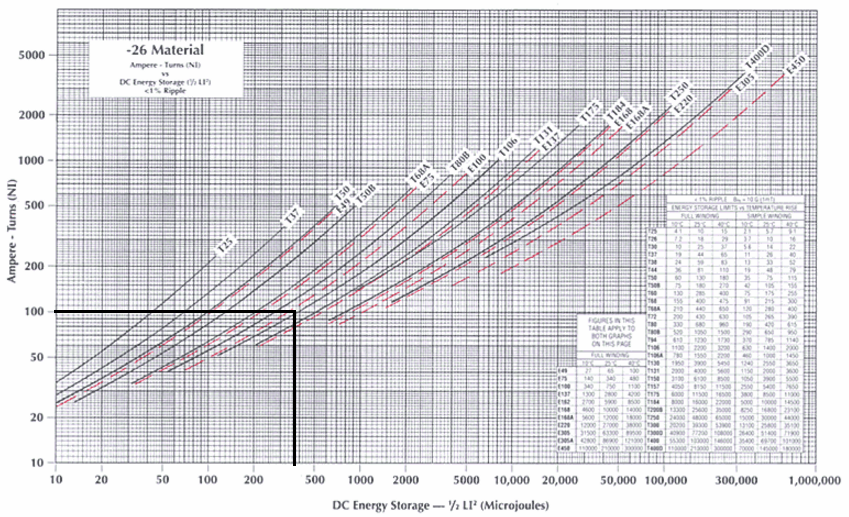
\includegraphics[width = 12 cm]{Imagenes/NIvsE}
	\caption{Ampere-Vueltas vs Energía para material n°26}
	\label{NIvsE}
\end{figure}

Para corroborar este valor obtenido, se calcula el número de vueltas a partir del $A_L$ proporcionado por el fabricante a partir de la ecuación \ref{A_L}.

\begin{equation}
L = A_L \cdot N^2
\label{A_L}
\end{equation}

\[N = \sqrt{\frac{L}{A_L}} = \sqrt{\frac{120 \; \mu Hy}{93 \; nHy/N^2}} = 35,92 \; vueltas\]

Se observa que los resultados son aproximados. Para asegurarse el valor deseado de inductancia se realizan 40 vueltas sobre el núcleo y se mide L con un punte RLC agregando o quitando vueltas hasta lograr el valor deseado. En el caso del núcleo utilizado en la práctica con 43 vueltas se logra una inductancia:
\[ L = 121,7 \; \mu Hy\]

La sección del conductor $S_C$ de cobre esmaltado a utilizar se determina teniendo en cuenta la corriente que circula por el mismo y la densidad de corriente $J$, en este caso se supone $J = 4,2$ $\frac{A}{mm^2}$.
\begin{equation}
S_C = \frac{I}{J}
\label{S_C}
\end{equation}
\[S_C = \frac{2,5 \; A}{4,2 \; A/mm^2} = 0,59524 \; mm^2 \; \]

El diámetro del alambre de cobre a utilizar es:
\[S_C = \pi \cdot (\frac{\phi}{2})^2 \; \rightarrow \; \phi = 2 \cdot \sqrt{\frac{S_C}{\pi}} \]
\[\phi = 2 \cdot \sqrt{\frac{0,59524 \; mm^2}{\pi}} = 0,870 \; mm \]

Por último, queda corroborar que la cantidad de vueltas con el alambre del diámetro calculado entre en el núcleo toroidal seleccionado. Para ello se calcula la sección de ventana $S_V$ del mismo (\ref{sv}) y se debe cumplir la relación \ref{relacionsvsc}.

\begin{equation}
S_V = \frac{\phi_{externo} - \phi_{interno}}{2} \cdot H_{toroide}
\label{sv} 
\end{equation}

\[S_V = \frac{26.9 \; mm - 14.5 \; mm}{2} \cdot 11.1 \; mm = 68.82 \; mm^2\]

\begin{equation}
S_V \geq S_C \cdot N
\label{relacionsvsc}
\end{equation}

\[68.82 \; mm^2 \; \geq 0,59524 \; mm^2 \cdot 43 \; vueltas \]
\[68.82 \; mm^2 \geq 25,595 \; mm^2 \]

\subsubsection{Capacitor}
El capacitor de filtrado de salida se determina con la expresión \ref{CO}. Sin embargo en la práctica se usan varios capacitores en paralelo y de distintas tecnologías para disminuir la $ESR$.

\begin{equation}
C_{min} = \frac{I_{omax} \cdot t_{offmax}}{\Delta V_{ripplemax}} = \frac{3.5 \; A \; \cdot 3.125 \; \mu s}{400 \; mV_{pp}} = 27.35 \; \mu s
\label{CO}
\end{equation} 

Se utilizan 3 o mas capacitores de $10$ $\mu F$ en paralelo.

\subsection{Circuito Final}
En la figura \ref{fuente} se observa el conexionado final de las distintas etapas antes calculadas.

\begin{figure}[H]
	\centering
	\includegraphics[angle = 90, height = 23 cm]{Imagenes/Circuito}
	\caption{Fuente conmutada half bridge.}
	\label{fuente}
\end{figure}

\section{Mediciones}
Las siguientes mediciones se realizaron con la fuente funcionando en las siguientes condiciones:
\begin{itemize}
	\item Tensión de salida: 24.8 V
	\item Corriente de salida: 2.48 A
	\item Carga fija y resistiva pura: 9.6 $\Omega$
	\item Potencia: 61.504 $W$
	\item Tiempo de funcionamiento: 10 minutos	
\end{itemize}

Luego se realizó una segunda medición con la fuente funcionando en las condiciones que se observan en la Fig. \ref{VIfunc} durante aproximadamente 30 minutos, obteniendo las mismas formas de onda que en el caso anterior. Para aumentar la corriente de salida lo que se hizo fue utilizar una resistencia variable y disminuir su valor hasta lograr la corriente deseada.
\begin{itemize}
	\item Tensión de salida: 24.4 V
	\item Corriente de salida: 2.976 A
	\item Carga variable: 8.2 $\Omega$
	\item Potencia: 72.614 $W$
	\item Tiempo de funcionamiento: 30 minutos	
\end{itemize}

\begin{figure}[h]
	\centering
	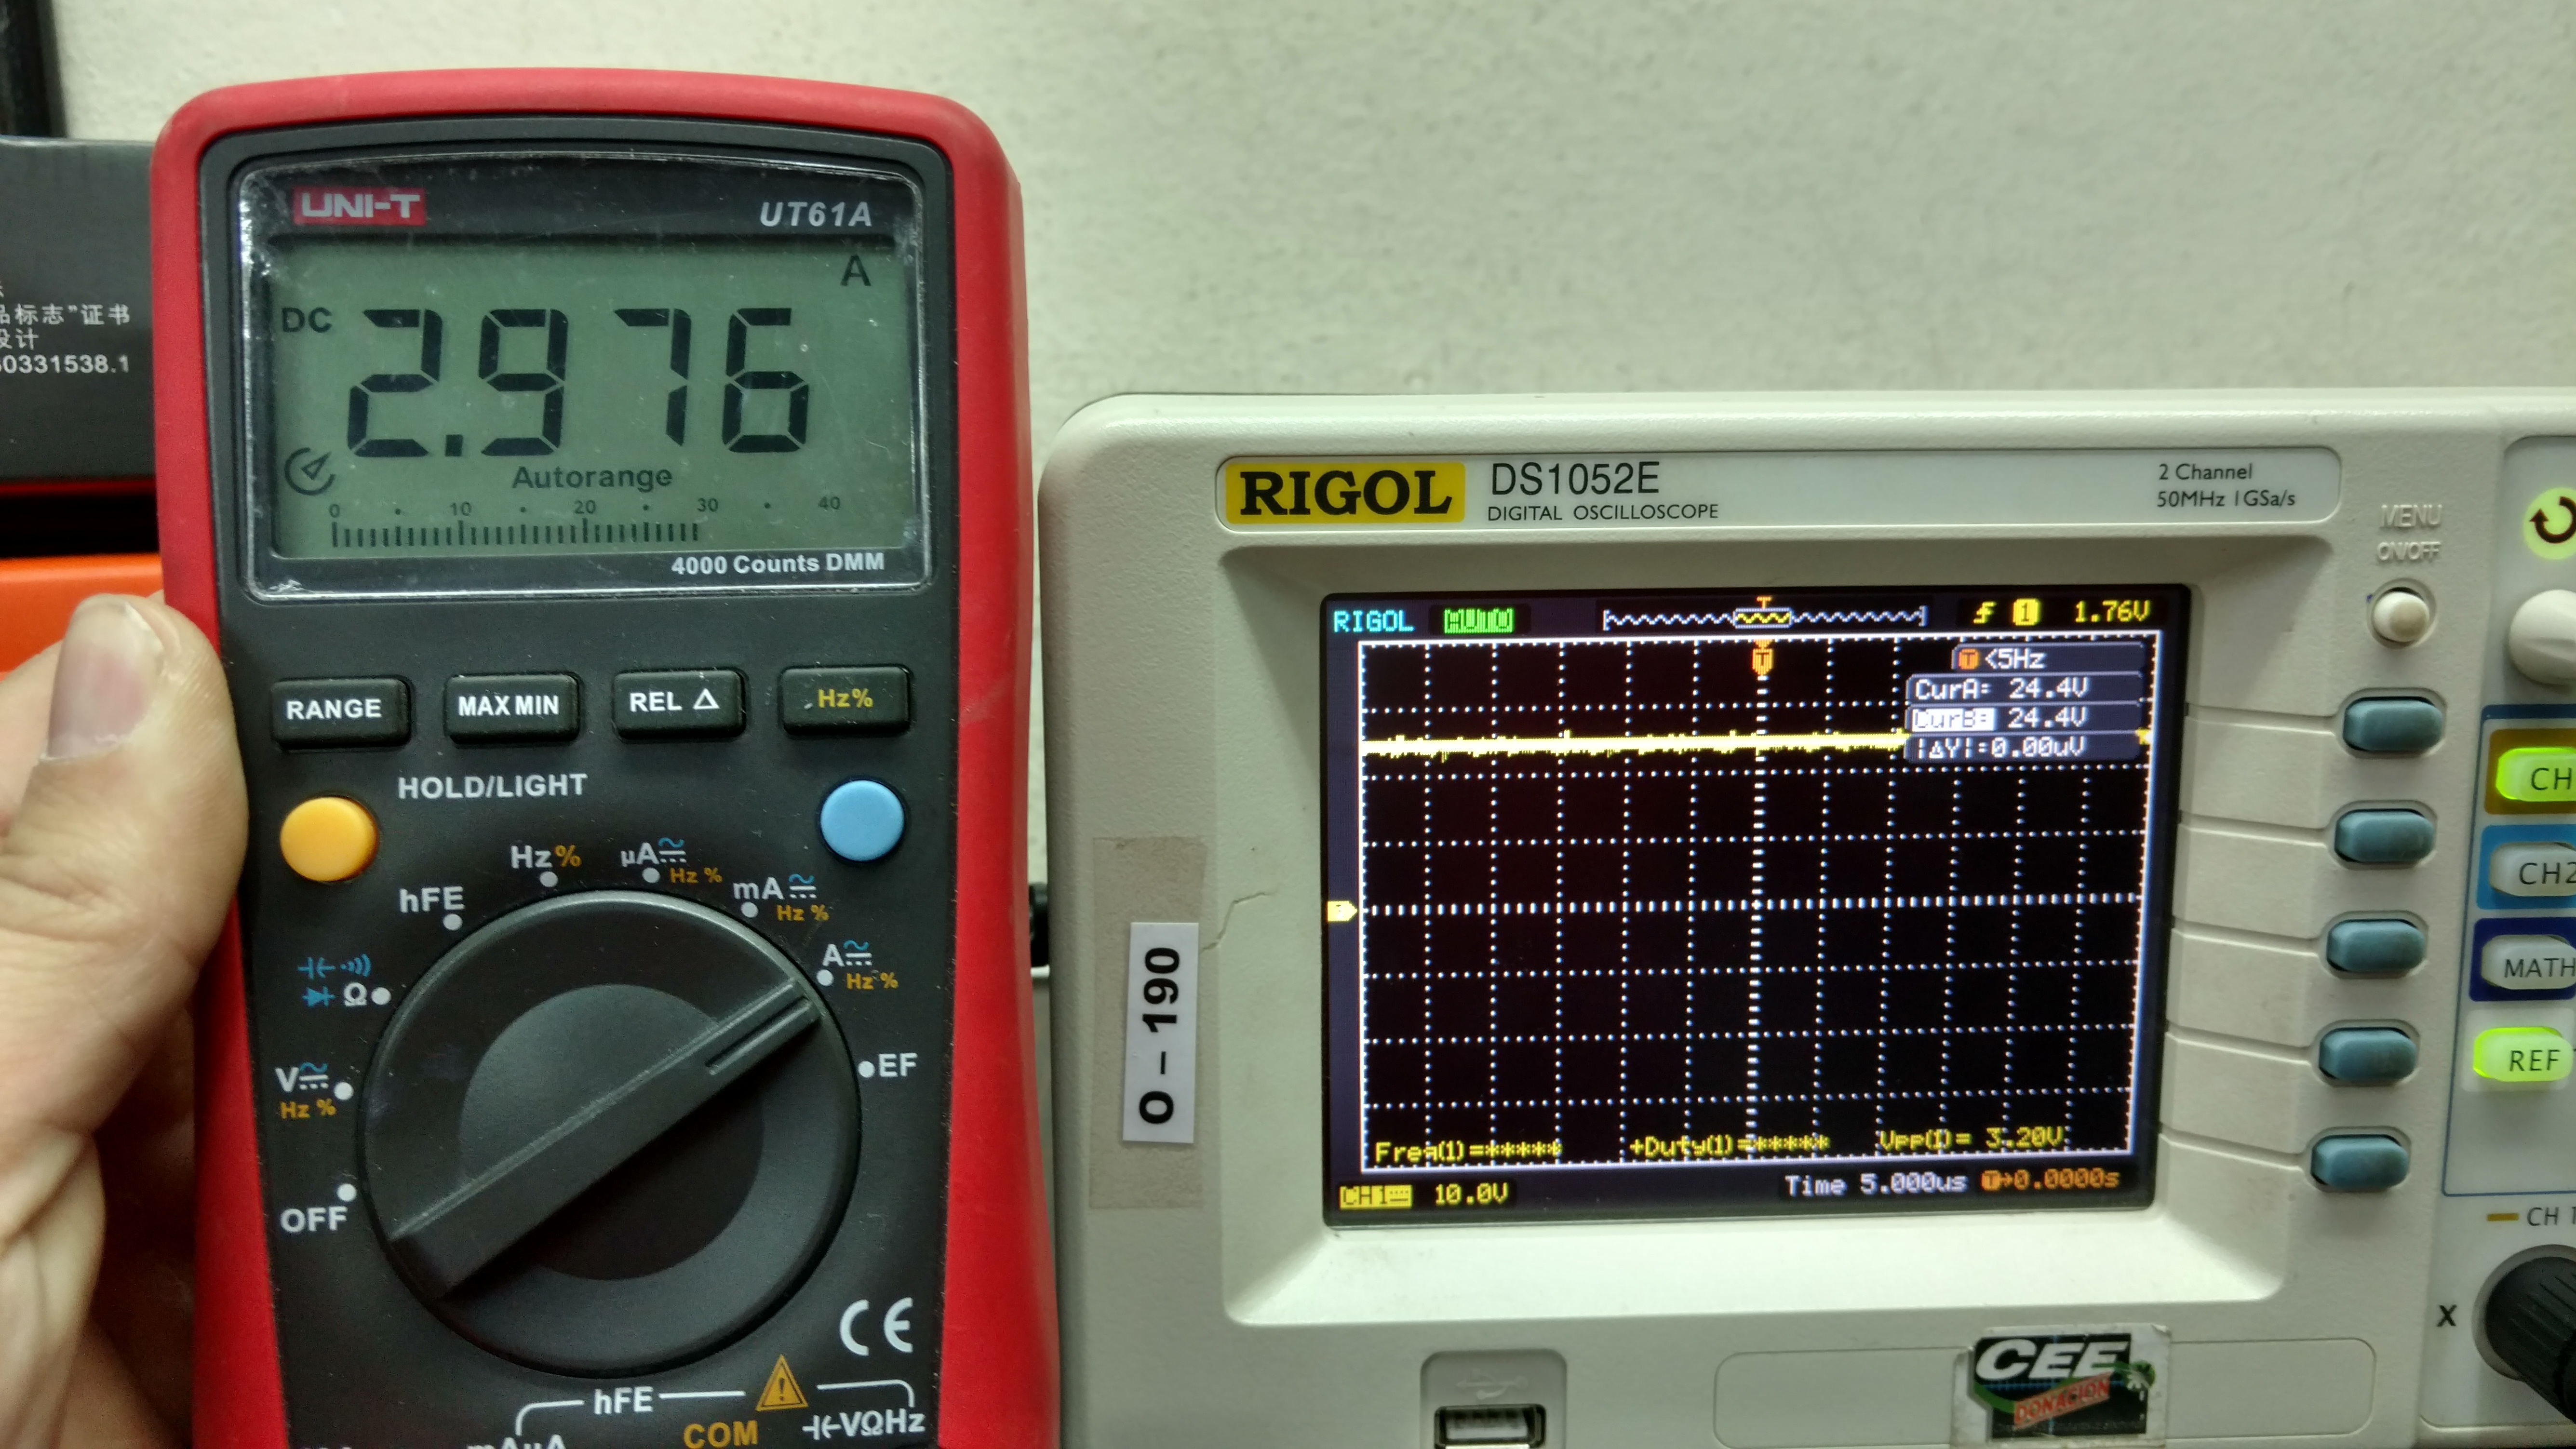
\includegraphics[width = 8 cm]{Imagenes/VIfunc}
	\caption{Tensión y corriente de salida de la fuente conmutada en prueba de 30 minutos de duración.}
	\label{VIfunc}
\end{figure}

\subsubsection{Tensión de salida CC}
\begin{figure}[H]
	\centering
	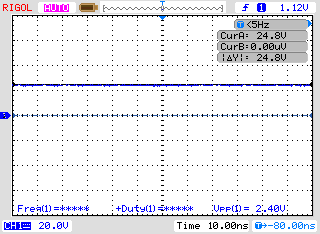
\includegraphics[width = 8 cm]{Imagenes/Vout}
	\caption{Tensión de salida de la fuente conmutada.}
	\label{Vo}
\end{figure}
\[V_{out} = 24.8 \; V\]

\subsubsection{Ripple de la Tensión de salida CA}
\begin{figure}[H]
	\centering
	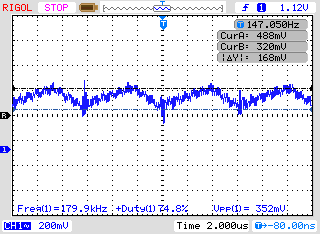
\includegraphics[width = 8 cm]{Imagenes/Ripple}
	\caption{Ripple de la tensión de salida de la fuente conmutada.}
	\label{Ripple}
\end{figure}
\[\Delta V_{Ripple} = 200 \; mV \; aprox.\]
\subsubsection{Señal de comando del PWM}
\begin{figure}[H]
	\centering
	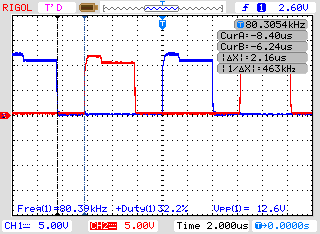
\includegraphics[width = 10 cm]{Imagenes/spwm}
	\caption{Señal de salida del SG3525.}
	\label{sPWM}
\end{figure}
En la Fig. \ref{sPWM} se observa la señal de mando del driver de los MOSFETs de potencia. En color azul está el canal A, en color rojo el canal B. Se observa además el tiempo muerto establecido entre pulsos, como así también la frecuencia de los pulsos y el duty cicle.
\[ t_{muerto} = 2.16 \; \mu s \]
\[ f_c = 80 \; KHz\]
\[ D\% = 32.2 \% \]

\subsubsection{Tensión de compuerta y de drenador de los MOSFETs}
En la Fig. \ref{VGDS} se observa la tensión de gate y de drenador (en ese orden) del MOSFET superior. La medición se realizó respecto de la tensión de surtidor de este transistor que es una masa virtual debido a las características de funcionamiento del driver de los transistores.

En la Fig. \ref{VGDI} se observa la tensión de gate y de drenador (en ese orden) del MOSFET inferior. La medición se realizó respecto de la tensión de surtidor de este transistor que es la masa del circuito.

En ambos casos se observa cuando el transistor pasa del corte a la saturación y el tiempo muerto existente.
 
\begin{figure}[H]
	\centering
	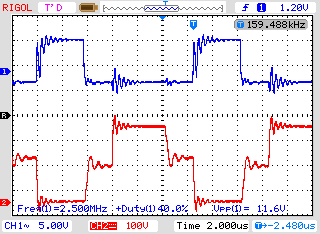
\includegraphics[width = 8 cm]{Imagenes/VGDs}
	\caption{$V_{GS}$ y $V_{DS}$ mosfet superior.}
	\label{VGDS}
\end{figure}

\begin{figure}[H]
	\centering
	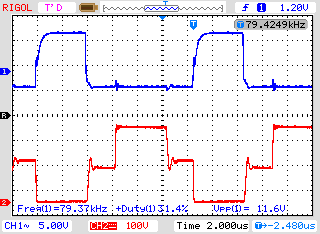
\includegraphics[width = 8 cm]{Imagenes/VGDi}
	\caption{$V_{GS}$ y $V_{DS}$ mosfet inferior.}
	\label{VGDI}
\end{figure}

\subsubsection{Primario del transformador}
\begin{figure}[h]
	\centering
	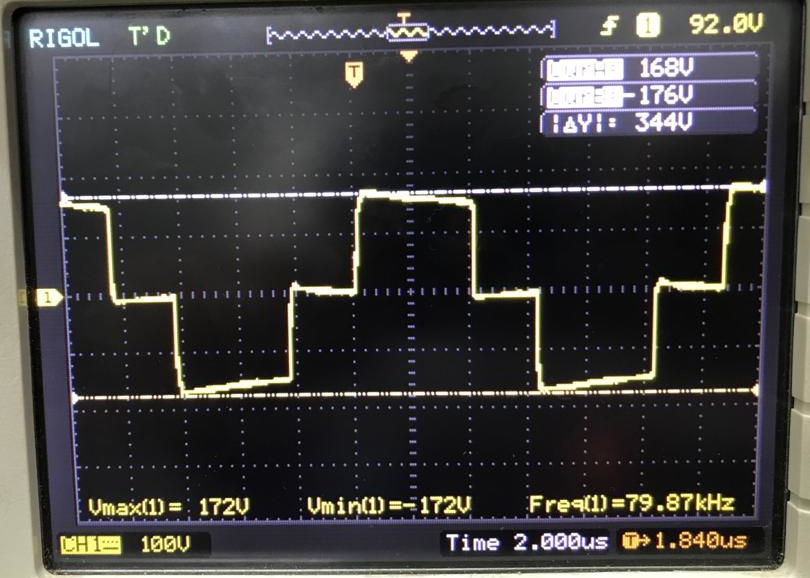
\includegraphics[width = 8 cm]{Imagenes/Vprim}
	\caption{Señal en el primario del transformador.}
	\label{primario}
\end{figure}

\section{Conclusiones}
A la hora del cálculo y diseño de la fuente conmutada no se encontraron mayores inconvenientes, pero si es necesario destacar las siguientes consideraciones:
\begin{itemize}
	\item Se utilizó el driver IR2110 para el manejo de los transistores, por una cuestión de simplicidad de diseño. El uso de este integrado simplifica la construcción del transformador de aislación para el manejo de los MOSFETs, evitando así los sobrepicos de tensión que se observaron en el trabajo práctico N° 3 de esta materia.
	\item El transformador de potencia a la salida del circuito, debe ser bobinado lo mas cuidadosamente posible para que las espiras queden parejas, evitando que haya distorsión en la señal a la salida de este y que los bobinados calienten de más.
\end{itemize}

En primer lugar, se procedió al armado de la fuente en 4 placas distintas interconectadas entre si. Estas placas contenían los siguientes circuitos: Filtro EMI + Rectificador, PWM, Driver + Transistores y Circuito de Salida. El trabajar con cuatro placas distintas presentó ciertas ventajas como la facilidad de discriminar el correcto o incorrecto funcionamiento de cada una da las partes del circuito y la sencillez de revisar el estado de las placas al no tener tantos componentes cada una. Sin embargo, el hecho de que el PWM, el driver, los transistores y el transformador de salida no estuviesen en una misma placa hacia que el circuito sea muy susceptible a interferencias. Por esta razón finalmente se implementó la fuente conmutada en dos placas, una con el filtro EMI y el rectificador y otra con el PWM, el driver y el transformador de salida.

Hay que resaltar en el diseño de la placa que contenga el driver, que la longitud de las pistas que conectan el driver con el gate del transistor debe ser la misma para ambos transistores, de acuerdo con la nota de aplicación del integrado, para evitar que haya un desfasare mayor al deseado entre señales. Además, cualquier señal de alta tensión deberá estar lo mas lejos posible de las pistas de gate para evitar que haya interferencia y que se disparen los gates en tiempos no deseados.

Para la prueba de funcionamiento de la fuente conmutada lo que se hizo fue en primer lugar corroborar que el PWM y el driver de los transistores estén funcionando correctamente. Luego se procedió a alimentar con corriente alterna desde una fuente variable a la etapa de rectificación y comprobar la correcta conmutación de los transistores. Aquí fue muy importante la comprobación de la señal en el primario y secundario del transformador de potencia, ya que en un primer momento los secundarios se encontraban bobinados en sentido opuesto haciendo que ambos conduzcan simultáneamente, lo que producía una menor potencia de salida. Por último, se colocó un disipador en los diodos rectificadores de salida debido al gran aumento de temperatura que este sufrió. Queda pendiente el análisis de elevación de temperatura para calcular el disipador adecuado a la aplicación.

De las diferentes mediciones efectuadas con la fuente en funcionamiento se concluye lo siguiente:
\begin{itemize}
	\item El ripple de tensión de salida se encuentra dentro del valor calculado. Los picos de tensión introducidos por la conmutación no tienen una magnitud considerable.
	\item La señal de disparo de gate del transistor inferior es mucho mas limpia que la del transistor superior. Esto se debe a que el transistor inferior se encuentra referenciado a la masa del circuito, mientras que el superior a una masa virtual. Además se observa claramente en las señales correspondientes al transistor superior la interferencia que produce la conmutación del otro transistor. Esta interferencia debe ser la menor posible de lo contrario se volvería a disparar el transistor superior estando el inferior disparado produciendo un cortocircuito. Para que este pico de tensión sea lo menor posible, las pistas del driver hacia los gates de los transistores deben tener la misma longitud y estar lo mas separadas posibles. Además se debe procurar que ninguna pista de alta tensión se encuentre cerca de estas pistas para evitar inducción de picos de tensión.
	\item Se observa en la señal de tensión drenador surtidor de los transistores, que la tensión máxima que estos soportan es $V_{in}$, característica de la fuente conmutada Half-Bridge.
	\item Respecto a la tensión medida en el primario del transformador de salida, se observa que el momento en que la tensión es máxima ($V_{in}$), el transistor superior se encuentra conduciendo y el inferior bloqueado. Cuando la tensión es mínima ($0 \; V$) el transistor superior está bloqueado y el inferior conduce y cuando la tensión es $\frac{V_{in}}{2}$ es porque ambos transistores están bloqueados, debido al tiempo muerto entre conmutación. En el tiempo muerto entre disparo de transistores se observó en un principio la presencia de un transitorio con picos elevados de tensión los cuales crecían a medida que aumentaba la tensión de alimentación de la fuente. Este transitorio se debe a que el transistor en cuestión no se apaga correctamente, haciendo que para elevadas tensiones de entrada este se vuelva a disparar produciendo un corto circuito con el transistor que si se encuentra conduciendo. La solución a esto fue emplear una red snubber en paralelo al primario del transistor sintonizada a la frecuencia del transitorio, por lo que $R = 56 \; \Omega \; 3 \; W$ y $C = 680 \; pF \; 500 \; V$. 
\end{itemize}

Para finalizar, se concluye que el diseño de una fuente conmutada es mucho más complejo que el de una fuente lineal, por lo que se debe ser sumamente cuidadoso a la hora de manipular los componentes electrónicos e instrumentos de medición, pero los resultados en cuanto a la eficiencia y potencia de la fuente son muy superiores, obteniendo un mejor aprovechamiento de la energía.


\end{document}
